\documentclass{standalone}
	\usepackage{tikz}
		\graphicspath{ {figures/AM_12_134/} }
	\begin{document}
\begin{tikzpicture}[node distance=0.01cm and 3cm]
 \node[anchor=center] (0) at (0,-0.8) { 12 \ (block5\_conv2) };
\node[anchor=center] at (6,-0.8) { 13 \ (block5\_conv3) };
 \foreach \label [count=\i] in {L11_F460.png,L11_F93.png,L11_F108.png,L11_F459.png,L11_F149.png,L11_F219.png,L11_F54.png,L11_F431.png,L11_F469.png,L11_F355.png,L11_F109.png} { 
 
	\node[draw=none] (\i) at (0,-\i*6em) {\includegraphics[width=0.3\textwidth]{\label} }; 
  }
\node[] (R) at (6,-6*6em) {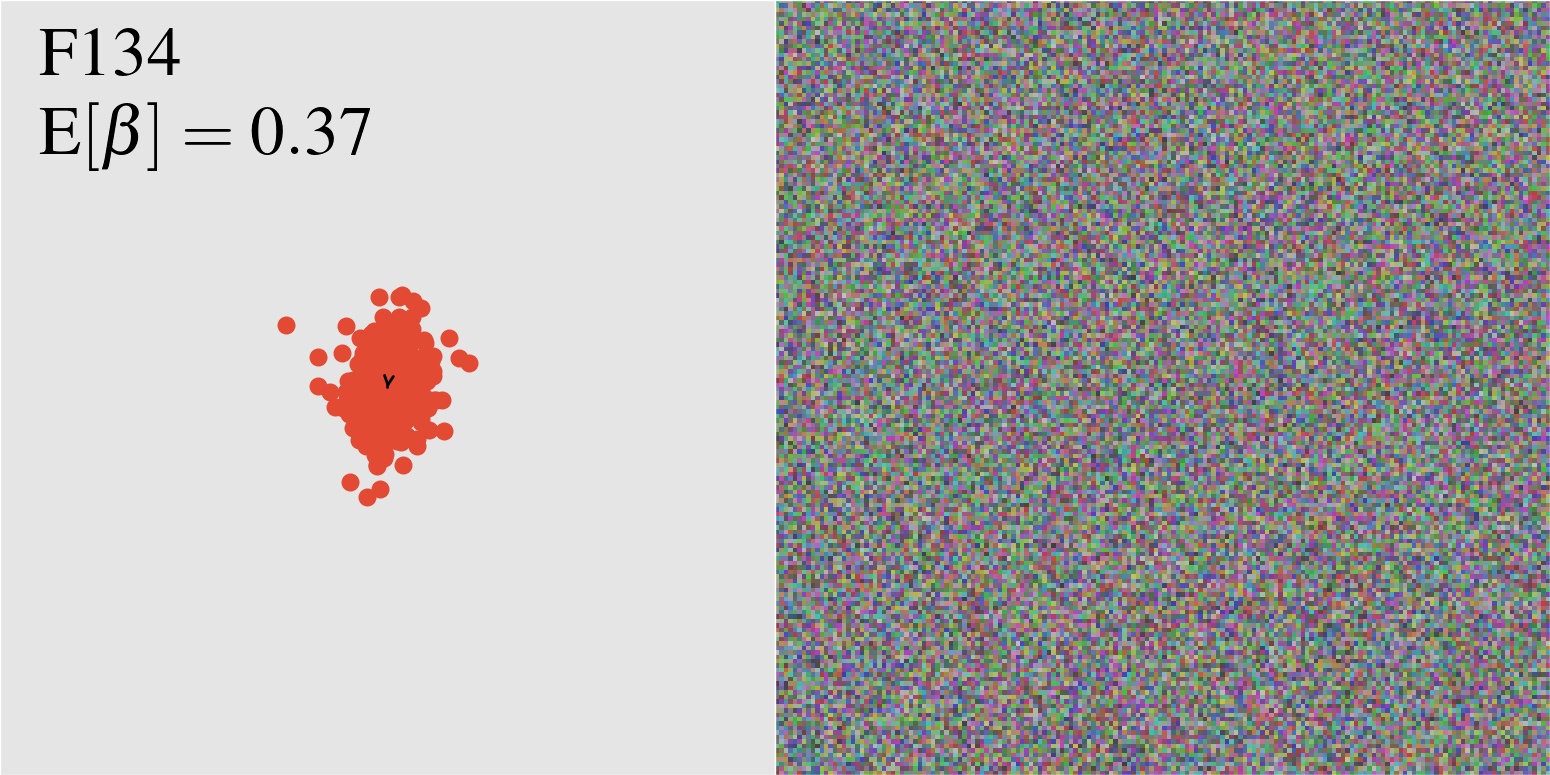
\includegraphics[width=0.3\textwidth]{ L12_F134.png } }; % Adjust the y-coordinate to center
 \draw (1.east) -- (R) node[pos=0.5, circle, draw, fill=white, minimum size=8pt, inner sep=0pt, scale=0.8] {$+$}; 
 \draw (2.east) -- (R) node[pos=0.5, circle, draw, fill=white, minimum size=8pt, inner sep=0pt, scale=0.8] {$+$}; 
 \draw (3.east) -- (R) node[pos=0.5, circle, draw, fill=white, minimum size=8pt, inner sep=0pt, scale=0.8] {$-$}; 
 \draw (4.east) -- (R) node[pos=0.5, circle, draw, fill=white, minimum size=8pt, inner sep=0pt, scale=0.8] {$+$}; 
 \draw (5.east) -- (R) node[pos=0.5, circle, draw, fill=white, minimum size=8pt, inner sep=0pt, scale=0.8] {$+$}; 
 \draw (6.east) -- (R) node[pos=0.5, circle, draw, fill=white, minimum size=8pt, inner sep=0pt, scale=0.8] {$-$}; 
 \draw (7.east) -- (R) node[pos=0.5, circle, draw, fill=white, minimum size=8pt, inner sep=0pt, scale=0.8] {$+$}; 
 \draw (8.east) -- (R) node[pos=0.5, circle, draw, fill=white, minimum size=8pt, inner sep=0pt, scale=0.8] {$-$}; 
 \draw (9.east) -- (R) node[pos=0.5, circle, draw, fill=white, minimum size=8pt, inner sep=0pt, scale=0.8] {$-$}; 
 \draw (10.east) -- (R) node[pos=0.5, circle, draw, fill=white, minimum size=8pt, inner sep=0pt, scale=0.5] { 1.0 }; 
 \draw (11.east) -- (R) node[pos=0.5, circle, draw, fill=white, minimum size=8pt, inner sep=0pt, scale=0.8] {$-$}; 
\end{tikzpicture}
\end{document}
